\chapter{Design and Implementation}\label{C:work}

A significant hurdle for the project was gaining enough understanding of the existing work on RBMs to be able to implement the ORBMs algorithm and architecture. This was crucial as an incorrect implementation invalidates  contributions \ref{item-c2} and \ref{item-c3} of this project.


\section{Implementation Design}

\begin{itemize}
  \item Ordering of evaluation tasks made unit testing, with hand made test cases possible. Also less risk, remove the uncertainty around the RBM.
  \item testing approach
\end{itemize}

\subsection{Language Choice}

\todowording{The implementation of the ORBM and inference algorithm is in \emph{Python}, with \emph{Matlab} and \emph{Java} being the other languages considered.}

I have spent my University career working in Java, and nowdays it is efficient to perform machine learning tasks. Python's module and class system promotes composition, and multiple inherietance in particular allows for composition of different classes.

Matlab is a popular numerical computing environment\todocite{} and has a lot of online resources as well as machine learing papers \todocite{} that include snippets or full Matlab programs that were used in the paper. Also Matlab is built around strong, efficient support for matrix operations which are very prolific in the RBM and ORBM implementations and evaluations.

Python has a very sucinct syntax and shallow learning curve\todocite{}, as well as being the langauge of choice of my supervisor. \todowording{This is favourable as I can have support for translating the algorithm into python correctly.} Through libraries that supply wrappers for C-bindings, efficient code can be written but overal being an interpreted language Python is slower than Matlab and Java\todocite{}. Three main factors influenced the choice for python:

\begin{description}
\item[Up front learning] Given the amount of up front learning of concepts required to implement the solution, Python was favoured over Java or Matlab because is has a very shallow learning curve. Despite having expeirence in Java as well as Python, I had never used machine learning or linear algerbra libraries in either languages. Given the amount of up front learning required to understand the concepts in this project let alone implement it, I opted for the shallower learning curve of Python. Also my supervisor has experience using Python and the libraries involved with this project. A shallower learning curve meant that more time could be allocated to the evaluation which is the foremost contribution of this project.
\item[Library Support] Matlab and Python were two contendors in this factor, as a lot of matlab machine learning code is avaliable with supporting papers \todocite{}. Python has libraries such as NumPy, SciPy and Matplotlib \todocite{} which mirror Matlabs functionality. However, NumPy and SciPy are all open source, while there is argument for treating an API as a black box --- i.e. not writing code that is dependant on the underlying implementation, having the option to view source helped me better grasp the concepts. In particular being able to compare my implementation of the RBM to Sklearn's \todocite{} allowed for some performance improvements.
\item[Ease of Evaluation] Python provides strong plotting library that is inspired by Matlab and R --- MatplotLib \todocite{}. Matplotlib is interoperable with the NumPy library, meaning that turning results into plots was really easy.

Also the evalation requires repeateldy running a test to gain more confidence in the stochastic result. This is made possible by the ECS-Grid \todocite{}. Python is supported with very minimal extra work required. A simple script that manages input and output is required. However the Java support on the ECS grid requires significantly more setup \todocite{}. \todowording{This seemed like an unnesccariy risk to introduce to the project at the later stage in the project where evaluation is being carried out.}
\end{description}
%
% All of the languages considered have the efficiency for machine learning tasks, despite Python being on the slower end of the spectrum of languages, versus that of the compiled JVM languages like Matlab or Java, it is still fast enough. The complexity of the traditional RBM is relative to what is trying to be modelled, less of the language implementing it.
% Java and Python have robust testing suites given they are used for non-academic goals. Matlab and R do have suites however the author has not had experience with them. Choosing from one of these two languages would increase the amount of upfront learning required and therefore increase this risk.
% The author had the most experience with Python and Java, however Python was favoured due to it's Matlab-like library NumPy. Expressive matrix syntax combined with the familiarity and brevity of Python made it a compelling option.


\subsection{Program Architecture}

The implementation of the RBM, ORBM and algorithm is implemented with unit testing and composability in mind. It is important that the design supports comparing the Full and Approximated Correction\todocite{Equation ..}. By using Python, multiple inheritance could be leveraged to achieve this composability. For instance  adding continuous pixel value support to the \texttt{Full Correction Sampler}, one simply needed to extend \texttt{Continuous Approximate Correction Sampler} and the  \texttt{Full Correction Sampler}, with no code actually in the new class. The architecture is pictured in the class diagram \ref{F:Prog-Arch}. There were three main roles these classes filled:
\begin{enumerate}
  \item The \texttt{Trainer} was used to train the weights of a supplied \texttt{RBM}. It would do so using a supplied \texttt{sampler}, decoupling how samples were generated from the training process.
  \item The \texttt{RBM} was the model of an RBM, storing the weight matrix, as well as parameter information. Also this supported conversion of the SciPy Sklearn libraries' RBM implementation into the implementation used in this project. Decoupling the concept of an \texttt{RBM} from the \texttt{Sampler} and the \texttt{Trainer} meant that RBMs could be `plugged` into the ORBM architecture with ease.
  \item The \texttt{Sampler} defined how to perform Gibbs sampling, the subclasses defining whether it is standard RBM sampling or ORBM sampling. This made is trivial to compose samplers, which was required for the ORBM samplers.
\end{enumerate}

\begin{figure}[h]
\begin{center}
  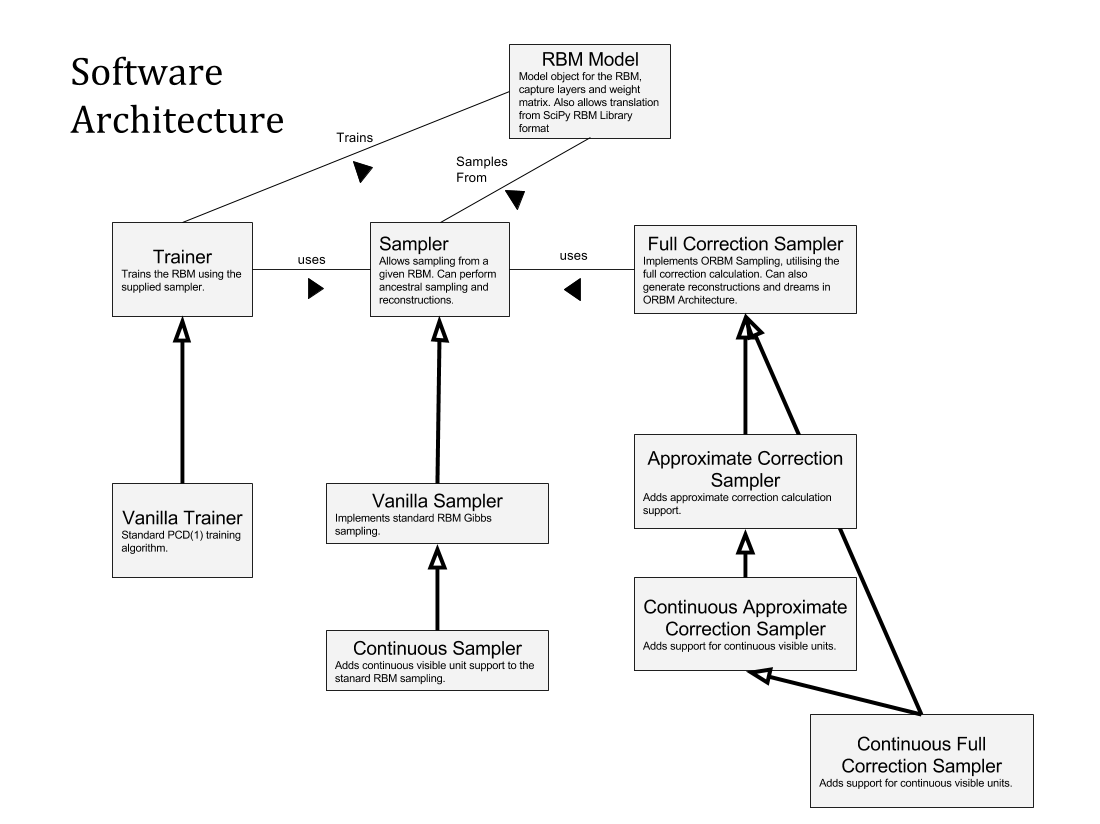
\includegraphics[width = 1\textwidth]{Assets/ENGR489-Architecture.png}
\caption{A figure showing the architecture for the implemented test suite in UML notation.}
\label{F:Prog-Arch}
\end{center}
\end{figure}

\subsection{Testing Approach}

The inference algorithm is the most crutial part of the implementation to test. In larger dimentional tasks, unit testing to ensure the algoruhtm produces the correct values becomes difficult. In smaller cases I was able to ensure the probabilities of $P(h|v)$ and $P(v|h)$ calculated by the implementation matches calculations I made by hand. Being an unsupervised black boxes, determining if an RBM (and by extension the ORBM) hidden representation is `correct` for larger tasks such as the MNIST handwritten digit dataset is non-trivial. Concerned by this risk, I designed my evaluations to build confidence in the algorithm and the implementation.

\section{Evaluation Design}

\subsection{Examining the mixing time of inference in the ORBM}

As described in Section \todocite{\ref{}}, sampling from $h^A$ and $h^B$ suffers from the effect of explaining away (\todocite{\ref{}}) which requires a Gibbs chain to run. While intractable for a large SBN, as only two causes are being modelled, ideally the Gibbs chain for this process won't take many iterations to mix. As the correction needs to be computed for each Gibbs iteration, a long Gibbs chain could be detrimental to performance.
Finding this \emph{optimal mixing time} for the ORBM is only an issue as the number of dimensions and training examples increase. In smaller dimensions mixing can be overcome by using a large ($>1000$) number of Gibbs iterations. However in the larger problems this becomes intractable, so an optimal mixing time is desired.

This project examines the mixing time by way of examining reconstructions at various points of the Gibbs chain. This is also interesting in that we can observe the dynamics of the network and the effect of apply the \emph{correction} has on reconstructions. \todocite{Hinton has shown this in practice as a useful thing to observe, cite his movies.}.

\subsection{Evaluating RBMs and ORBMs}

  A challenge faced by this project and work with RBMs is that they are non-trivial to evaluate \todocite{}. Being unsupervised black box, one cannot merely inspect the hidden units for an input and be sure that a good model has been learnt. As I plug RBMs into the ORBM architecture it is important for the overal results that the RBMs are well trained.

\subsection{Hinton diagrams}
  We can examine the weights into a given hidden unit in the shape of the visible vector. For instance in the context of images, \texttt{Hinton Diagrams} allow visualisation of what a given hidden unit is `doing` by visualising the matrix. This was first used by Hinton in the context of Boltzmann Machines in \cite{Hinton:1986:LRB:104279.104291}. They also give insight into hidden unit utilisation. Weights are often initialised to small random values resulting in a Hinton diagram with little structure to it. This is illustrated in figures \ref{F:Hinton-Good} and \ref{F:Hinton-Bad}. The former showing a hidden units weights where some structure has been learnt, and the latter showing the opposite.

  \begin{figure}[htb]
  \centering
  \begin{subfigure}[t]{0.3\textwidth}
      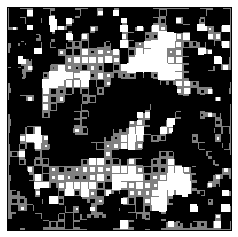
\includegraphics[width=\textwidth]{Assets/HINTON1.png}
      \caption{Utilised hidden unit Hinton Diagram}
      \label{F:Hinton-Good}
  \end{subfigure}
  ~ %add desired spacing between images, e. g. ~, \quad, \qquad, \hfill etc.
    %(or a blank line to force the subfigure onto a new line)
  \begin{subfigure}[t]{0.3\textwidth}
      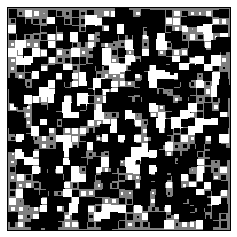
\includegraphics[width=\textwidth]{Assets/HINTON2.png}
      \caption{Unutilised hidden unit Hinton Diagram}
      \label{F:Hinton-Bad}
  \end{subfigure}
  \caption{Hinton Diagrams illustrating a trained hidden unit, versus that of an untrained/unutilised hidden unit. This is with no measures to enforce sparsity.}\label{fig:mnist-worse-best-results}
\end{figure}

\subsection{Reconstructions: a measure of performance}

Reconstructions, as described in Section \ref{SS:RBM-Reconstructions}, are a good measure of performance. \todocite{Hinton showed this in papers, also cite more ppapers showing reconstruction use. starting from early RBM training papers by Hinton, up to more recent in deeper networks - the goal being to show the reader that reconstructions are used well in practice.} Given the precident for using reconstructions as a performance measure, they will be the main way I evaluate the RBM in comparison to the ORBM. To be able to use this reconstruction based evaluation, knowledge of the ground truth was required. This was so:
\begin{itemize}
  \item RBMs could be trained and then plugged into the ORBM network.
  \item Reconstructions could be compared directly (by score) to the ground truth.
\end{itemize}



\subsection{Evaluating RBMs: Problem dependent}

  Evaluating RBMs is problem dependant, we can examine the different approaches avaliable by splitting problems into two cases:
  \begin{description}
  \item[Problems with small dimentionality] When the dimentionality of the input is very small ($<10$) and all possible inputs are known we can perform analytical evaluations of the RBM. By clamping the visible units of the RBM to each input in the training set, reconstructions can be created. This process can be repeated for each input, recording the frequency that each reconstruction occurs on a bar graph. We can then ensure that the RBM is reconstructing the input perfectly. For instance, an RBM trained on two bit XOR and clamped to the input $[1,0]$, might have a bar graph of reconstructions as illustrated in figure \todocite{\ref{F:Two-Bit-RBM-Recons}}.

  In a similar way to the reconstructions, samples can be drawn from RBM in a `free phase` without the input clamped to a given visible. The bar graph should exhibit dream visible patterns from the whole training set approximately an equal amount. Using the two bit XOR example once more, an example bar graph is shown in figure\todocite{\ref{F:XOR-ORBM}}.


  \begin{figure}[htb]
  \centering
  \begin{subfigure}[t]{0.4\textwidth}
      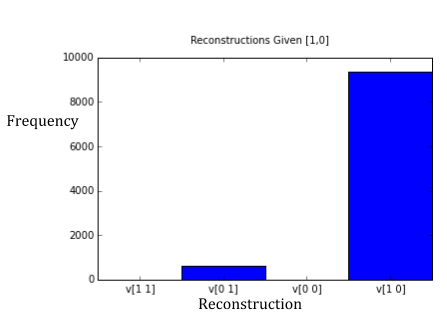
\includegraphics[width=\textwidth]{Assets/Two-Bit-RBM-Recon.png}
      \caption{Example reconstructions for the Handcrafted RBM, For 10000 independant reconstructions given the input $[1,0]$.}
      \label{F:Two-Bit-RBM-Recons}
  \end{subfigure}
  ~ %add desired spacing between images, e. g. ~, \quad, \qquad, \hfill etc.
    %(or a blank line to force the subfigure onto a new line)
  \begin{subfigure}[t]{0.4\textwidth}
      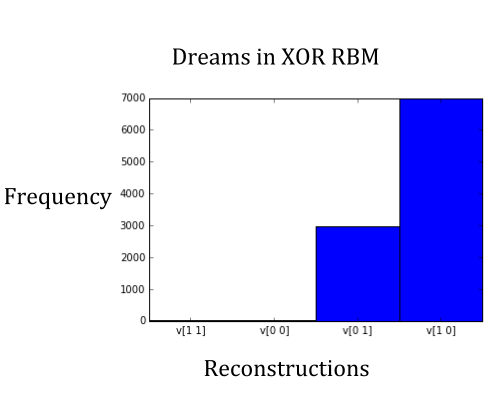
\includegraphics[width=\textwidth]{Assets/XOR-RBM-Dreams.png}
      \caption{Dreams in the XOR RBM, note how only the training data is present.}
      \label{F:Two-Bit-RBM-Dreams}
  \end{subfigure}
  \caption{Bar graphs exmplifying the use of reconstructions and dreams for small numbers of RBMs.}\label{F:XOR-Example-Plots}
\end{figure}


  \item[Problems  with large dimentionalities] In non-trivial cases, with larger datasets, reconstructions can be inspected and compared to the training dataset. However, empirically detecting if a model is trained is difficult, especially given the unsupervised, black box nature of RBMs.
  Alternatively, a `score` can be assigned to each item in the training set based on how well the RBM can reconstruct it. However in large cases your training set will not be complete --- you will not have every possible valid image like you would in a case where your images are 2 pixels.
  Dreams can also be examined in larger cases, but emperically detecting if they are `correct` is infeasible. Nevertheless, Dreams are useful to examine as dreams that look like items in the training set gives confidence the RBM \todowording{has learnt something.}

\end{description}


\todowording{My \todowording{x experiements} all followed the same high level process, working from trivial cases to more challenging tasks. The reason for this being that trivial cases make unit testing feasible, therefore ensuring conclusions can be drawn with regard to the algorithm and model, not an incorrect implementation.} By incrementally increasing the difficulty of the task, it allows me to identify what qualities of the problem make the algorithm less or more effective.

The evaluations in this project aimed to evaluate the ORBM and it's inference algorithm by examining reconstructions given a \todowording{multi-subject image}. Because the multi-cause inputs were images composed of known images, I could then compare the reconstructions to the ground truth. An example of a multi-cause input with two quadrilaterals is shown in figure \ref{F:Composite-Example}. The optimal reconstructions are equivalent to the two images that combined form the input.

\begin{wrapfigure}{r}{0.6\textwidth}
  \begin{center}
    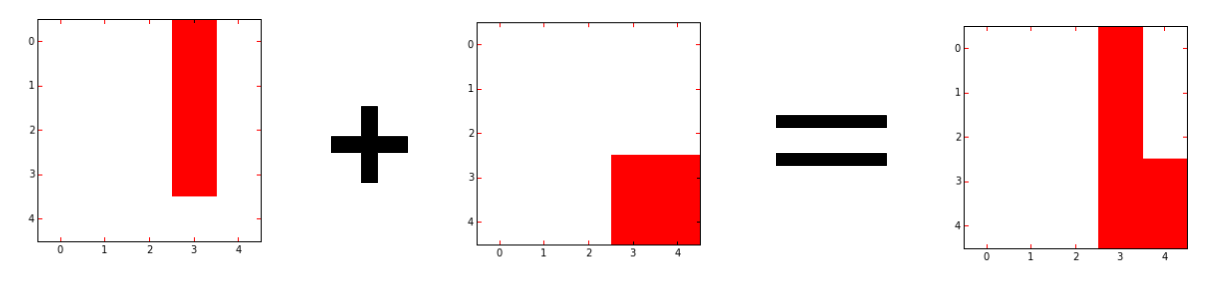
\includegraphics[width=0.48\textwidth]{Assets/Composite-Example.png}
  \end{center}
  \caption{A figure illustrating two five by five pixel images combining to form a composite/multicause input. The images are binary.}
  \label{F:Composite-Example}
\end{wrapfigure}

In the smaller dimenisonal cases the reconstructions are inspected by plotting the reconstructions and the frequency with which they occurred after a large amount of repetitions. In the larger dimensional tasks, two `scores` are used to evaluate reconstructions against the corresponding item of the training set.



\subsection{Choice of Evaluation Datasets}

As my evaluations follow the same outline of training RBMs, pluging them into the ORBM, and evaluating the reconstructions, the aspect of the evaluation that needs to be designed is the datasets for these tasks. It is important the images of the datasets are \emph{multi-subject} and that the individual images used to compose the training images are known. This is to allow the reconstructions of the ORBM (and RBM) can be compared to these underlying images, exploring how well the ORBM and RBM can perform source separations.

\begin{itemize}
  \item 2 Bit XOR --- The minimal case of image source separation. The RBMs are trained on a single bit being on in a two bit pattern. The training set then resembles a 2 bit XOR truth table. Because the dimensions of this task are so small, reconstructions and dreams can be evaluated emperically. Also the algorithm can be unit tested ensuring the outputs of the different steps are correct, comparing them to values calculated by hand. Also as the dimensionality is so small, the Approximated Correction \todocite{\ref{}} and the Full Correction \todocite{\ref{}} can be compared to ensure that the approximated correction works well in practice.
  \item $X$ neighbouring bits on in $Y$ bit pattern --- This is a natural next step from 2 bit XOR, and is effectively the same task but in larger dimensions. It is trivial to train an RBM to represent this problem, and the algorithm is quick to run on such a small dimensonality creating a quick feedback loop for development.
  \item 2 by 2 squares in a 5 by 5 pixel image --- This dataset extends the previous increasing to 25 dimensions. The dataset is trivial to construct and corresponds to a square of 2 by 2 pixels being on in a 5 by 5 pixel image. Interesting cases can be explored and then inspected visually as images, which are easier to interpret than bit strings (especially as the bit strings get larger than 10).
  \item Rectangles in a 5 by 5 pixel image --- This dataset builds on the previous by introducing different shaped \emph{subjects} to the images. This means that two RBMs need to be trained, one for each subject. This dataset, much like the previous allows for compelling cases to be separated. It sets the scene for the larger dimension cases.
  \item MNIST Handwritten Digit Dataset --- \todocite{MNIST} this is a prolific machine learning dataset \todocite{lots of papers please.}. By using the dataset in this project it aids in reproducibility of this project and as there has been previous work it is known that RBMs can be trained sucessfully on the data \todocite{MNIST RBM paper Hinton}. The dataset is comprised of 28 by 28 pixel handwritten digit images, where a pixel value is between 0 and 1. There are digits 0 through 9. For each digits it is composed with every other digit, making the novel, yet non-trival task of separating two digits from a single image.
\end{itemize}




% \subsection{Language Choice}\label{SS:language}
%
% The project is currently implemented using Python 3.4, however three other languages were considered for this project, Matlab, R and Java.
% Several factors were considered that lead to this decision.
%
% \begin{description}
% \item[Efficiency]A large amount of data is required to train a Restricted Boltzmann Machine and the new approach has a higher complexity than the traditional RBM implementation. The language choice should not prevent the algorithm from being run in reasonable time, as this would hamper the ability to test it for correctness and performance.
% \item [Ease of use]The project requires significant up front learning which means some familiarity with the language or a shallow learning curve will help keep velocity/progress high. The focus can then be on understanding the required theory instead of language niches.
% \item  [Support for testing]From a correctness standpoint, being able to evaluate the algorithms will require confidence of a correct implementation and therefore help lend credibility to subsequent findings.
% \item [Machine Learning Library support]Being able to leverage libraries allows the focus to be on implementing and testing the new algorithm.
% \item [Stakeholder collaboration]The projects supervisor who conceived the new approach inherently has a good understanding of how it works and therefore having a language they are comfortable working in can help with ensuring implementation correctness. For instance pair programming has been employed which is facilitated by a programming language common to both developers.
% \end{description}
%
% All of the languages considered have the efficiency for machine learning tasks, despite Python being on the slower end of the spectrum of languages, versus that of the compiled JVM languages like Matlab or Java, it is still fast enough. The complexity of the traditional RBM is relative to what is trying to be modelled, less of the language implementing it.
% Java and Python have robust testing suites given they are used for non-academic goals. Matlab and R do have suites however the author has not had experience with them. Choosing from one of these two languages would increase the amount of upfront learning required and therefore increase this risk.
% The author had the most experience with Python and Java, however Python was favoured due to it's Matlab-like library NumPy. Expressive matrix syntax combined with the familiarity and brevity of Python made it a compelling option.
%
% \subsection{Library Choice}\label{SS:Lib}
%
% Considerations regarding library choice only really apply to the part of the system that needs to be robust, the number crunching.
%
% Given the choice of Python, the decision to use the NumPy library was almost inherent. NumPy is a linear algebra library that offers fast implementations of matrix operations in a concise, expressive syntax. For instance, a whole training set of images, each image of size $ x^2 $, represented by a $ 3 $ by $ x$ by $x $ matrix, can then be operated on all at once. Also NumPy is interoperable with open source Python Machine Learning Libraries. For instance Scikit-Learn \cite{scikit-learn} and Theano \cite{bergstra+al:2010-scipy} which allows greater reproducibility in my results. Finally, it is a mature, well tested library, being an evolution of the Numeric python library which started developing in 1995 \cite{2015HistSciPy}.
% %
% \subsection{Dataset Choice}
%
% A crucial part of the project is ensuring that the tests can be reproducible, allowing any results to be used as evidence in a paper. Hence the importance of choose a dataset that has some credibility or can allow this approach to be compared to existing work. The MNIST digit dataset was originally chosen as a good dataset for this projects tests. There has been work using RBMs \cite{Hinton:2006dk} and other machine learning approaches \cite{Lecun:1998hy},  to represent these handwritten digits previously. This gives a point of reference to compare performance.
%
% It is worth noting: In section \ref{SS:HDR} it is highlighted that the results from testing with this dataset are not outstanding, hence a more minimal toy-dataset is being used until more understanding can be gained about what is and is not working.
%
% \section{Implementation}\label{S:Implementation}
%
% The traditional Restricted Boltzmann Machine has been implemented.
%
% The new theory applies a correction when constructing the hidden representation of the noisy input. This correction allows each model (RBM) to take responsibility for different parts of the input data.
%
% The calculation of this correction introduces a dependency between the hidden units and therefore we sacrifice some efficiency for better performance on multi-cause data.
% The full, un-approximated correction calculation has been implemented and connected to the Restricted Boltzmann Machine.
%
% Tests have been created to verify if the new approach is working.
% As RBMs are generative models, we can show them an input and have them generate their own recreation based on the internal representation. This recreation is dependant on the image it was created from and therefore could be used for a performance test.
% We can approximate the likely-hood of, given a noisy image, how well can we reconstruct the underlying clean image. This forms a 'score' for the $ith$ pixel of an image.
%
% $$  P( v_i' | v_i^{composite}) = P(v_i' | v_i^{clean}  ) $$
%
% Where $ v_i' $ is the reconstruction based on the RBMs internal representation. $ v_i^{composite} $ is the composite (noisy) image and $ v_i^{clean} $ is the clean image; the underlying model that noise is added to to create the composite image.
%
% This score can then be approximated image-wise and compared to the traditional approach, by sampling (creating reconstructions). From this we can see which images the new approach performs better/worse.
%
% \subsection{Handwritten Digit Recognition}\label{SS:HDR}
%
% The performance tests described in section \ref{S:Implementation} have been implemented for all digits in the MNSIT Handwritten Digit dataset \cite{mnistlecun} and the results are not outstanding. A toy model of a horizontal bar acts as the noise and is composed with the digit dataset to create the noisy input. We see this in \ref{F:digit_example}. The Noisy Input is the composite image, this is what the reconstructions pictured in New Approach and Traditional Approach were generated from. The target was generated from the underlying (non-composited) '2' images.
%
% \begin{figure}[htbp]
% \begin{center}
% 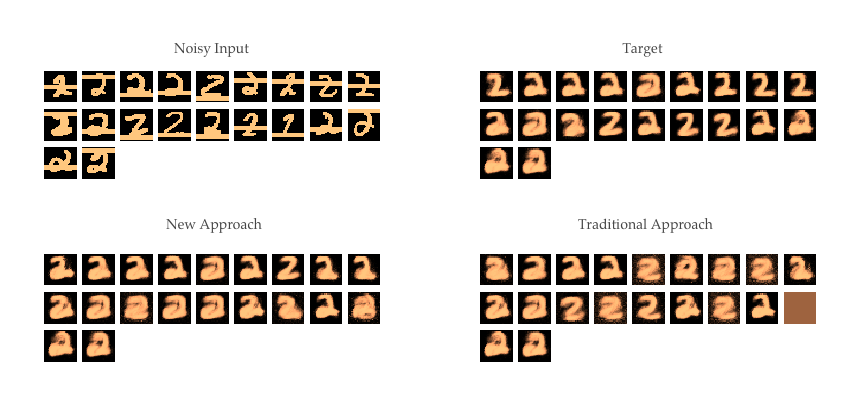
\includegraphics[width=1\textwidth]{Assets/Initial_Results}
% \caption[Initial results using new approach on noisy handwritten two images.]{Initial results using new approach on noisy handwritten two images. The input was 20 MNIST two digits with a random 4 pixel high bar composited. The new technique does not perform better by much over the dataset.  }
% \label{F:digit_example}
% \end{center}
% \end{figure}
%
%
% Another performance test carried out has been classification performance. The hypothesis being that the new approach should be able to generate a better representation despite having noisy training and test sets. The actual classification is deferred to an AI classifier that is trained on the hidden representations.
% Fig \ref{F:rbmClassification} shows a visual representation of this. The RBM is trained on some data, then a hidden representation and known labels are used to create a transformed training and test set which a perceptron or other classifier is then trained on. The better the classification performance the better representation the model has achieved.
% \begin{figure}[htbp]
% \begin{center}
% 	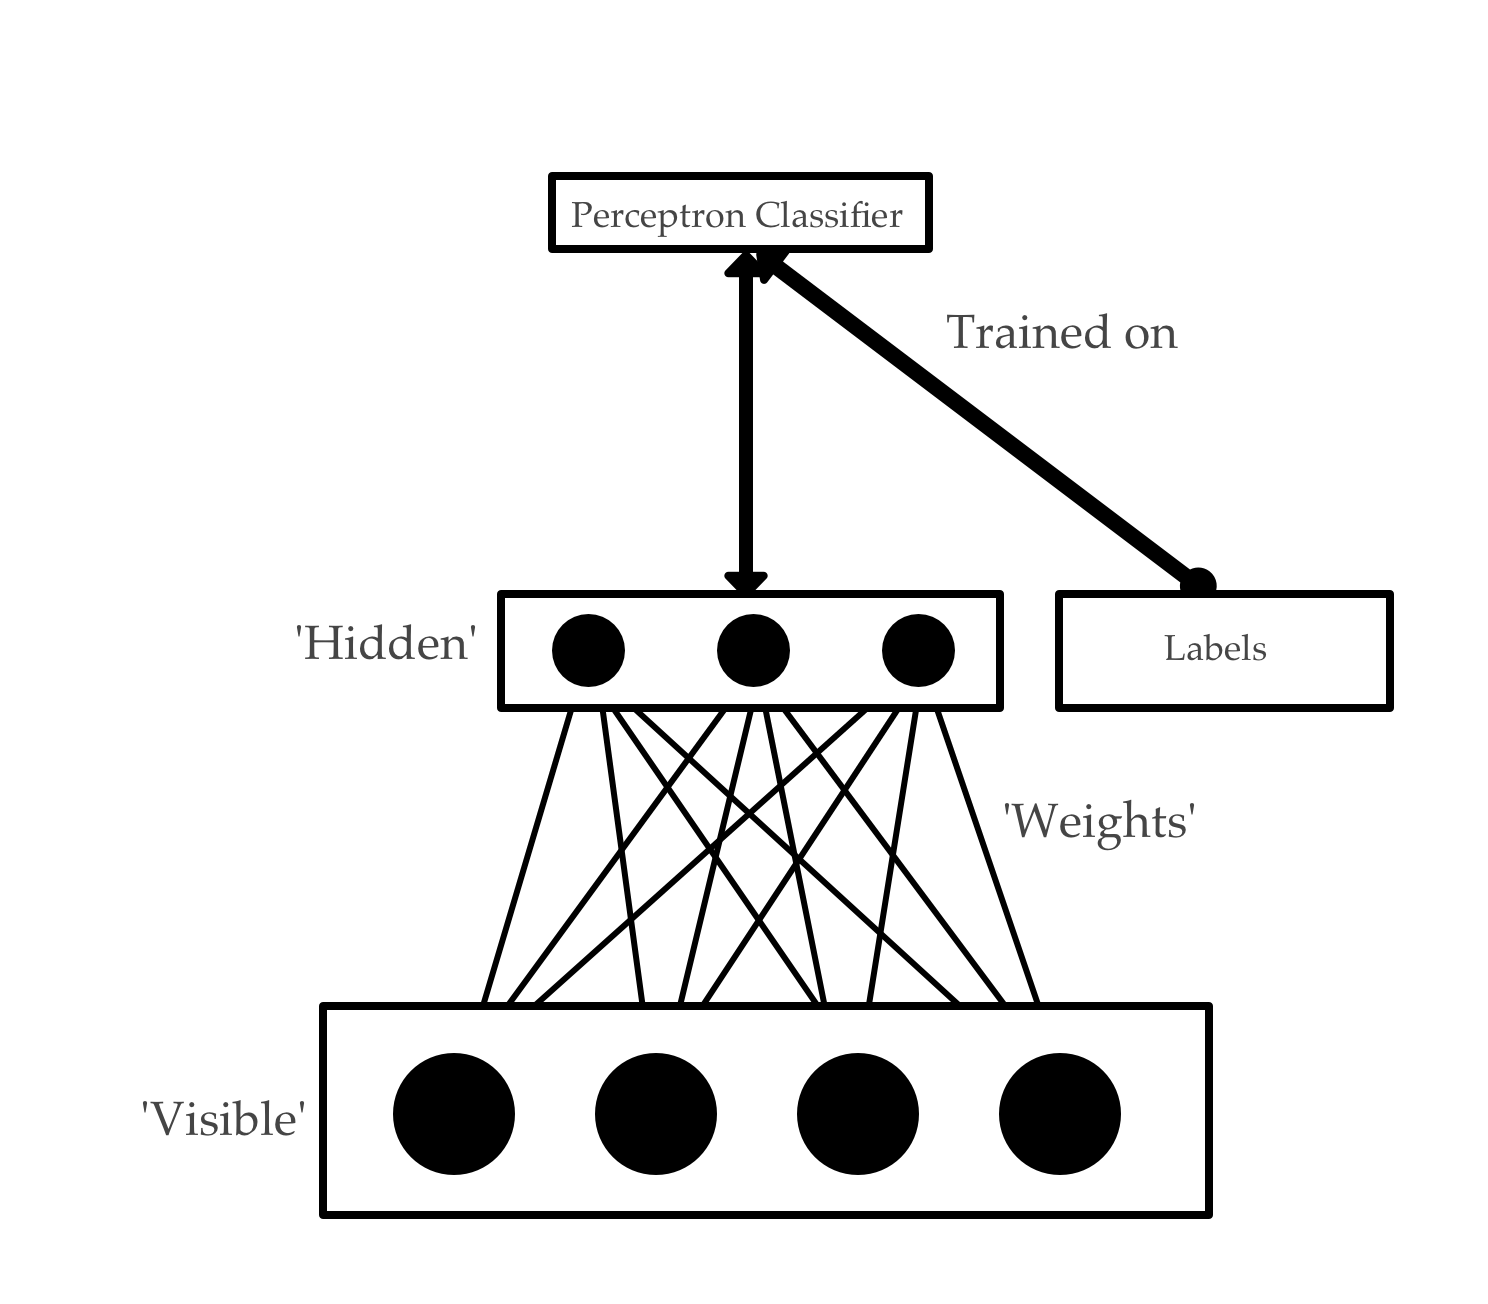
\includegraphics[width=0.7\textwidth]{Assets/RBMClassification}
% \caption[Figure demonstrating how classification can be applied using an RBM]{Figure demonstrating how classification can be applied using an RBM. }
% \label{F:rbmClassification}
% \end{center}
% \end{figure}
%
% \begin{figure}[htbp]
% \begin{center}
% 	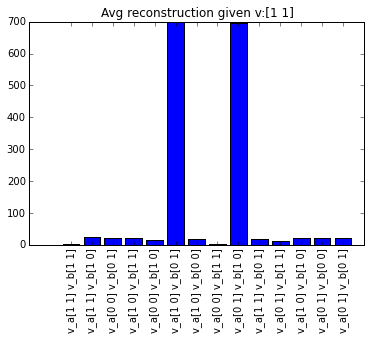
\includegraphics[width=0.7\textwidth]{Assets/yup}
% \caption{Figure showing the results of generating reconstructions using the new approach and two identical RBMs that can recognise a single pixel being on a time.}
% \label{F:twobit}
% \end{center}
% \end{figure}
%
% The non-outstanding results shown in \ref{F:digit_example} and the other digits, highlighted that some minimal test cases need to be satisfied before more complicated models like digits can be explored. The tests currently in place are not atomic enough.
%
% We arrived at the minimal test case, a two bit image, with binary pixels and a toy RBM model trained to understand one pixel being on at a time. This had the advantage of being able to be checked by hand and approximations of the correction could be explored in the minimal case. This is the  smallest case possible for them to actually work and as a result, more robust correction tests have been constructed.
%
% In the two bit scenario it is very easy to measure the performance of reconstructions, we would hope given an visible input of $ v = [1,1] $ that the new approach would most of the time result in reconstructions from the two models of $ v'_A = [1,0]$,  $v'_B = [0,1] $ and conversely $ v'_A = [0,1]$,  $v'_B = [1,0] $. Where $v'_A$ is the reconstruction generated, given $v$ from model A.
%
% The results of doing this in a two bit system, that is two hidden and two visible units resulted in the plot in fig \ref{F:twobit}. We see the most common reconstructions are those defined above. It is important to look at the reconstructions from both models holistically to ensure they are actually separating the sources. The figure shows the average of 1000 runs of the new approach, the two bit example making this many runs quite feasible with so few features.
%
%
% \section{Evaluation Planning}\label{S:evaluation}
%
% As the output of the project is essentially a series of reproducible performance results, it is important that the algorithm is sound in practice and matches what the theory describes. The validity of the results hinge on the confidence that the code does what it should. This precondition is enforced by unit and integration testing the system. The third party libraries in use for linear algebra (NumPy) and plotting (Matplotlib) are well tested and feature in other peer reviewed literature in the field of Machine Learning \cite{Millman:2011wp}.
%
% As touched on in the scope changes in section \ref{S:ScopeChanges} the evaluation phase of the project needs to be ongoing. The performance of the new approach needs to be checked at every point to ensure that cases where the new approach does and does not work can be pinpointed. It also makes tracking down what factors make it more or less effective easier.
% The actual approach to evaluation is touched on above, but it amounts to verifying if and when the new approach generates a better representation of a composite image versus that of the traditional approach.
